\documentclass[12pt, a4paper, one side]{article}
\usepackage[utf8]{inputenc}
\usepackage[french]{babel}
\usepackage{biblatex}
\usepackage{listings}
\usepackage{xcolor}
\usepackage{hyperref}
\usepackage{graphicx}
\usepackage{minted}

\bibliography{reference}

\usepackage{comment}

\lstset{
    basicstyle=\itshape,
    xleftmargin=3em,
    literate={->}{$\rightarrow$}{2}
        {^}{$\uparrow$}{1}
        {↓}{$\downarrow$}{1},
    morekeywords={method_body, decl_method, type, ident, list_params, multi_line_string, METHOD_BODY, STRING_LITERAL},
    basicstyle=\small
}

\definecolor{codegreen}{rgb}{0,0.6,0}
\definecolor{codegray}{rgb}{0.5,0.5,0.5}
\definecolor{codepurple}{rgb}{0.58,0,0.82}
\definecolor{backcolour}{rgb}{0.95,0.95,0.92}

\lstdefinestyle{mystyle}{
    commentstyle=\color{codegreen},
    keywordstyle=\color{magenta},
    numberstyle=\tiny\color{codegray},
    breakatwhitespace=false,
    breaklines=true,
    captionpos=b,
    keepspaces=true,
    numbers=left,
    numbersep=5pt,
    showspaces=false,
    showstringspaces=false,
    showtabs=false,
    tabsize=2,
    extendedchars=true
}

\newcommand{\paragraphln}[1]{\paragraph{#1}\mbox{}\\}



\title{Documentation de l'extension}
\author{}
\date{}

\begin{document}

    \maketitle

    \begin{center}
        Valentin Laclautre, Anthony Dard, Damien Trouche, Martin Gangand, Basel Darwish Jzaerly
    \end{center}

    \tableofcontents

    \newpage

    \section{Spécifications}

    A noter que vous devez disposez au minimum de la version 1.8 de java pour
    pouvoir faire tourner les programmes deca compilés en bytecode java.

    \subsection{Compilation de programmes deca en exécutable pour la JVM}
    \subsubsection{Commande decac}
    \textbf{decac -java [-n] [-d]* [-P] [-w] $<$fichier deca$>$...}
    \\

    L'option -java spécifie au compilateur qu'on souhaite compiler un programme deca en exécutable pour la machine virtuelle Java.
    Ainsi, on obtient avec cette option un fichier .class exécutable par la JVM au lieu d'un fichier .ass (exécutable IMA). Les conventions de nommage sont les mêmes, c'est-à-dire que le nom du fichier compilé est celui du programme deca, seule l'extension du fichier change.

    Cependant il y a quelques restrictions. En effet, l'utilisation de code Java dans une méthode Deca impose une compilation vers la JVM (une erreur est renvoyée sinon). De plus la compilation vers la JVM impose qu'il n'y ait pas de méthode en assembleur. (cf Limitations pour plus de précisions)

    \subsubsection{Spécification de compilation}
    La compilation se fait de la même manière que pour la machine IMA au détail près qu'au lieu d'appeler nos méthodes de compilation pour la machine abstraite IMA, le compilateur utilise la bibliothèque ASM\cite{ASM} pour la génération du bytecode.

    \subsubsection{Compiler un programme Deca}

    Pour compiler un fichier deca, il suffit simplement de taper : \newline
    \textbf{decac -java <path>/<fich>.deca}

    \subsubsection{Fichiers créés par la compilation}

    Lors de la compilation d'un fichier deca, un premier fichier correspondant
    au programme principale portant le même nom que le fichier deca est créé (mais
    avec l'extension .class au lieu de .deca), puis un fichier portant le nom
    MethodBody est créé. Ce fichier permet de gérer l'insertion de java en deca
    (pour plus de précision, veuillez regardez la section consacrée). Enfin pour
    chaque classes deca contenue dans ce fichier, un fichier .class est créé avec
    le même nom que le nom de la classe. Ce fichier correspond au bytecode de la
    classe deca.

    \subsubsection{Exécuter des fichiers deca}

    Après avoir compilé un fichier deca (nommé pour l'exemple \textit{fich.deca})
    on aimerai pouvoir l'exécuter. Pour cela, il faut se placer dans le répertoire
    du fichier deca (là où les fichiers .class se sont créés) et il faut taper :
    \newline \textbf{java fich}. On peut aussi taper \textbf{java -cp path fich} où path correspond au chemin du fichier deca.

    \subsection{Appel de code Deca en Java}

    Après avoir créée une classe en deca, et l'avoir compilé en un fichier .class,
    il est possible de l'instancier dans une classe java. Malgré tout, pour pouvoir
    faire cela, il faut placer le fichier java et le fichier deca au même endroit.
    Après l'avoir instancié, on peut l'utilisé de la même maniere qu'une classe
    java, et faire appel à des méthodes ou des champs de la classe deca.

    \subsubsection{Exemple de Deca vers Java}

    Dans cet exemple, il y a 2 fichiers: un fichier deca comportant une classe, et
    un fichier java instanciant cette classe. \newline
    \newpage
    \textbf{Math.deca}
    \begin{minted}{java}
        class Math {
        	int add(int a, int b) {
        		return a + b;
        	}

        	int mult(int a, int b) {
        		return a * b;
        	}
        }
    \end{minted}

    \textbf{Main.java}
    \begin{minted}{java}
        class Main {
        	public static void main(String[] args) {
        		Math m = new Math();
        		int c = m.add(1, 2);
        		System.out.println(c);
        		c = m.mult(5, 3);
        		System.out.println(c);
        	}
        }
    \end{minted}

    Pour compiler, il ne reste plus qu'à copier les lignes suivantes :
    \begin{minted}{bash}
        $ decac -java Math.deca
        $ javac Main.java
    \end{minted}

    Ces deux commandes compilent dans un premier temps le programme deca, puis
    dans un second temps le programme principale java. Enfin, il ne reste plus qu'à
    exécuter le programme :

    \begin{minted}{bash}
        $ java Main
        3
        15
    \end{minted}

    \subsubsection{Intérêt d'avoir du code Deca vers Java}

    Cela permet un portage très simple pour les développeurs ayant décidé
    d'utiliser le langage java et ayant besoin d'utiliser une éventuelle librairie deca.
    Le langage deca étant neuf, un portage du langage vers java serait un atout attrayant pour les développeurs.

    \subsection{Appel de code Java en Deca}
    Cette section précise les spécifications liées à l'appel de code Java en Deca.
    \subsubsection{Grammaire Deca pour l'appel de code Java}
    Un mot clé est ajouté au lexer \textbf{'java'} permettant de préciser que la méthode contient du code java de la même manière que les méthode écrite en assembleur.

    La syntaxe est enrichie de la règle suivante:
    \begin{lstlisting}
decl_method -> type ident '(' list_params ')'
            java '(' multi_line_string ')' ';'
    \end{lstlisting}
    La règle de décompilation devient donc:
    \begin{lstlisting}
METHOD_BODY^r -> MethodJavaBody[ STRING_LITERAL^code ]
                { r := "java(".code.");"}
    \end{lstlisting}
    Ainsi, une règle est également ajoutée à la passe 3 pour prendre en compte les méthodes Java
    \begin{lstlisting}
method_body↓env_type↓env_exp↓env_exp_params↓class↓return
            -> MethodJavaBody [ StringLiteral ]
    \end{lstlisting}

    Comme pour les méthode écrite en assembleur, aucune vérification de code n'est faite sur la portion en Java, il appartient donc au programmeur de s'assurer que le code est correct. Dans le cas contraire, des erreurs du compilateur Java  ou encore des erreurs à l'exécution sur la JVM peuvent être levées.

    \subsubsection{Utilisation}
    L'utilisation de l'appel de code Java en Deca est très similaire à l'appel de code assembleur. En effet, il suffit de déclarer une méthode de la même manière, c'est-à-dire une méthode dont le corps est une chaîne de caractères contenant du code Java et en utilisant le mot clé 'java' à la place de 'asm'.
    \\

    Il est possible d'envoyer une valeur qui se trouve dans le code deca vers le code java en utilisant les paramètres de la méthode deca. Un exemple d'utilisation se trouve dans src/test/deca/codegen/valid/custom/extension/*.
    \\

    Enfin, il est utile de rappeler qu'il est possible de compiler une classe écrite en deca et puis utiliser le bytecode généré dans un programme java. On note que le fichier deca source doit être dans le même répertoire que le fichier java afin que la compilation fonctionne. C'est une limitation de deca.

    \newpage
    \section{Analyse bibliographique}
    Dans cette section nous allons donner des détails techniques sur la  \textbf{Java virtual machine JVM}.

    \subsection{Structure de fichier .class}

    \begin{figure}[h]
        \centering
        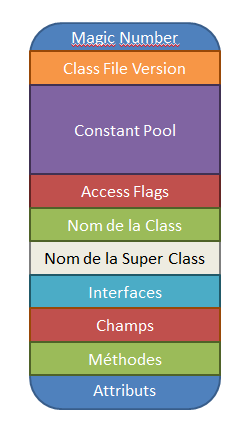
\includegraphics[scale=0.80]{JavaInternal.png}
        \caption{L'architecture de fichier .class \cite{ref_DexFormatvsJavabytecode}}
        \label{fig1}
    \end{figure}


    Les fichiers .class sont les fichiers exécutables par la machine virtuelle java. Chaque fichier .class contient les informations concernant une et une seule classe en Java. Dans ce fichier on trouve les instructions écrites en bytecode qui seront exécutées par la JVM. Nous présentons par la suite quelques détails, mais pour plus de détails il faut regarder les spécifications du java \cite{ref_specifications_java} .

    \subsubsection{Magic number}
    Il s'agit d'un attribut identifiant les fichiers d'execution Java \cite{ref_DexFormatvsJavabytecode}.

    \subsubsection{Class file version}
    Permet de déterminer la version minimum de la machine virtuelle de java qui pourra exécuter ce fichier. Donc si la version du fichier est supérieure à celle de la JVM, la machine virtuelle ne pourra pas l'exécuter.

    \subsubsection{Constant Pool}
    C'est une table qui contient toutes les constantes de la classe. Ces constantes peuvent être de types différents tels que \textbf{String},\textbf{Integer}, \textbf{Float}... etc. Par exemple, lorsque le fichier .java contient une variable qui a pour valeur 123456, cette table contiendra une case référencée par un indice et cette case stocke la valeur. De façon similaire, une chaîne de caractères telle que "ma belle chaîne de caractère" sera stockée dans une autre case dans la table.

    \subsubsection{Access Flags}
    Contient les informations sur l'accessibilité de la classe.

    \subsubsection{Class Name}
    On y trouve le nom de la classe.
    \subsubsection{Super Class Name}
    On y trouve le nom de la classe mère.

    \subsubsection{Interface}
    Si la classe implémente une interface, alors le nom de l'interface sera mentionné ici.

    \subsubsection{Champs}
    Les champs de la classe sont présentés ici avec leur niveau d'accessibilité private,protected ou public avec son nom et son type.

    \subsubsection{Methods}
    De façon similaire aux champs, chaque méthode est décrite par son niveau d'accessibilité, son nom, les types de ses paramètres et le type de retour.

    \subsection{Les types}
    Il existe deux sorts de type en java. Les types primitifs. L'autre sort est les types références. Une référence peut être de type classe ou de type tableau.
    \\

    On distingue ces types :
    \subsubsection{Les types numériques}
    Il existe deux catégories :
    \begin{itemize}
        \item Entier : tels que byte, short,int et char.
        \item A Virgule flottante : comme float et double.
    \end{itemize}

    \subsubsection{Le type boolean : } représente une valeur de vérité true ou false.
    \subsubsection{Le retour d'adresse : } le type returnAddress est un pointeur vers
    un des \textbf{Opcodes} de la JVM (utilisé par les instructions JSR, RET, et JSR$\_$W).

    \subsection{Les zones mémoires \cite{ref_zones_memeoire_java}}
    Il existe différentes zones de mémoire pour stocker les données pendant l'exécution d'un programme. Quelques zones sont crées au démarrage de la Java Virtual Machine et sont détruites quand elle s'arrête. Il existe d'autres zones qui sont crées lors de la création d'un nouveau thread, elles sont propores à ce thread et enfin détruites à la fin du thread.
    Nous allons détailler quelques zones :

    \subsubsection{Le registre program counter :} C'est un registre propre à chaque thread.

    \subsubsection{La pile d'exécution :} C'est une pile propre et privée à l'exécution de chaque thread. La pile est crée au moment de la création du thread et sera détruite à la fin du thread. Le rôle de la pile est de stocker les \textbf{Frames} que nous allons détailler dans la section suivante.

    \subsubsection{Le tas :} C'est une zone commune à tous les threads de la JVM. Il est créé au moment du démarrage de la JVM. Elle y stocke les données allouées dynamiquement telles que les instances des classes et les tableaux.

    \subsubsection{Zone de méthodes :}
    C'est une zone qui stocke le code de toutes les classes. Elle est partagée par tous les threads et elle stocke la \textbf{Constant Pool} \ref{Constant_Pool}, les champs et les variables de classe et des méthodes ainsi le code des méthodes.

    \subsubsection{Constant Pool : } \label{Constant_Pool} Pour chaque classe dans un fichier .class, il existe une table Constant Pool \ref{fig1}. Cette table est représentée dans une zone mémoire appelée Constant Pool. Elle contient toutes les constantes connues à la compilation et les références vers les méthodes qui doivent être résolues à l'exécution.

    \subsection{Les frames :}
    Une frame a pour rôle de stocker les données et les résultats partiels, on y stocke aussi la valeur de retour des appels aux méthodes. A chaque appel à une méthode, une nouvelle frame est crée. Elle sera détruite à la fin de l'appel. La freme est allouée dans la pile du thread qui l'a créé. Cette frame a son propre tableau de variables locales, sa pile d'opérandes et une référence vers la constant pool de la classe de la méthode appelée.

    \subsubsection{Les variables locales :}
    Chaque frame contient un tableau de variables locales. Une variable locale   simple en terme de taille peut contenir un type boolean, byte, char, short, int, float, reference, ou returnAddress. Pour stocker des variables locales de type double ou long, il faut la place de deux variables locales simples.
    Chaque variable est indexée par un indice. Comme dans une pile, l'indice de la première variable est 0. Les valeur des long ou double sont rangées dans deux cases consécutives.
    Lorsque une méthode statique est appelée, tous les paramètres sont passés dans des variables locales consécutives à partir de la variable locale d'adresse 0.
    Lorsque une méthode non statique est appelée, la référence sur l'objet à qui  est appelée a 0 pour indice de variable. Cette variable correspond à \textbf{this} en java. Les autres paramètres de la méthode seront rangés dans les cases qui suivent.

    \subsubsection{La pile des opérandes :} Chaque frame a une pile des opérandes.
    La JVM fournit des instructions pour charger des constantes ou des valeurs, depuis les variables locales dans la pile des opérandes.
    D'autres instructions récupèrent des opérandes provenant de la pile, réalisent une opération sur celles-ci, puis stockent le résultat dans la pile d'opérandes de cette frame.

    \newpage
    \section{Conception}

    La librairie utilisée pour créer le bytecode java est asm. Grâce aux classes
    et méthodes de la librairie, il est possible de décrire totalement le programme
    java à partir de l'arbre créé lors de la compilation. Le but de cette extension
    va donc être de redéfinir l'étape C.
    Cette section détail également les fonctionnalités d'utilisation de code Java en Deca et inversement.

    \subsection{Compilation deca pour la JVM}
    \subsubsection{Structure Globale}

    Pour écrire un fichier contenant du bytecode java, il faut utiliser les classes
    de la librairie asm, qu'il faut pouvoir utiliser à n'importe quel endroit dans
    l'arbre d'exécution. C'est le but de la classe \textbf{JavaCompiler} qui
    possède des attributs de type \textbf{ClassWritter} et \textbf{MethodVisitor}
    étant utilisés dans le programme. Ces attributs possèdent des getters et des
    setters, ce qui permet permet de les récupérer à n'importe quel endroit du
    programme, mais aussi de les modifier, par
    exemple quand une nouvelle méthode est créée, et que c'est une nouvelle
    instance de \textbf{MethodVisitor} qui
    rentre en vigueur. La classe \textbf{JavaCompiler} implémente de plus
    l'interface \textbf{Opcodes} d'asm. Cela permet de pouvoir utiliser à partir
    de \textbf{JavaCompiler} les opcodes du bytecode java lorsque cela est
    nécessaire. Enfin cette classe implémente une méthode permettant de créer le
    fichier .class du programme principale, mais aussi touts les
    fichiers .class des classes deca contenues dans le fichiers source, et le
    fichier permettant l'insertion de Java en Deca.

    Les fichiers utilisés pour la génération de code sont les mêmes qu'à la partie
    C, puisqu'il faut parcourir le même arbre après l'étape B. L'enjeu est donc
    de redéfinir les fonctions de l'étape C afin de les adapter à la génération
    de code en bytecode java.

    \subsubsection{Calcul de la taille de la pile des opérandes et des variables locales}

    A chaque définition de méthodes, il faut pouvoir donner la taille de la pile
    des opérandes et la taille du tableau de variables locales. La librairie permet
    de calculer automatiquement cela pour nous, il n'y a donc aucune classe
    à créer pour gérer cette partie.

    \subsubsection{Gestion de génération de code}

    Contrairement à la machine abstraite IMA, il n'y a pas de registre à gérer
    dans la JVM. Toutes les opérandes nécessaires sont prises sur la pile.
    En revanche toutes les variables sont stockées dans la table des variables
    locales. Il faut pouvoir stocker l'index dans cette table pour les identifier.

    \subsubsection{Sauvegarde des Identifier dans la table des variables locales}

    La tables des variables locales est très importante dans une méthode, car c'est
    elle qui stocke toutes les variables de celle-ci. Dans la fonction main, qui
    est une fonction statique, le premier élément stocké dans cette table est la
    liste d'arguments donnés en paramètres. Lors de la création de variables,
    un compteur est initialisé à 1 dans le main et est incrémenté à chaque
    déclaration de variable. Ce compteur correspond à l'index dans la table de variables locales de la variable courante. Il est mis à jour dans la définition
    de la variable qui possède un attribut sauvegardant cet index.

    Dans le cas où l'on se situe dans une méthode autre que main, la table des
    variables locales contient en premier lieu l'adresse de notre classe (ce qui
    correspond à this), si la méthode n'est pas statique (ce qui est toujours le
    cas en deca). Ensuite, cette table contient tout les paramètres de la méthode.
    Lors de la déclaration des paramètres dans les méthodes, on initialise donc
    l'indice à 1 que l'on incrémente selon le même principe que dans le programme
    principale. On met à jour aussi les informations dans la définition des
    paramètres. Ce n'est qu'ensuite dans le corps de la méthode, lors de la
    déclaration de variables, qu'on les stocke dans la table des variables locales,
    mais à un indice se situant après les paramètres de la méthode.

    \subsubsection{Méthodes de génération de code}

    Pour la génération de code, on reprend le même principe qu'à l'étape C. Pour générer des
    instructions, on fait appel à la méthode \textbf{codeGenInstByte}.
    Pour effectuer des opérations, il faut charger l'expression dans la pile
    des opérandes. C'est la méthode \textbf{codeGenExprByteOnStack} qui s'en
    charge. C'est la méthode principale de l'extension, qui est redéfinie partout,
    de la même manière que \textbf{codeGenExprOnRegister} pour la compilation
    vers IMA. Par exemple, pour un litteral, celui-ci est chargé directement
    dans la pile avec une méthode d'asm. Pour une variable, on charge son contenu
    dans la table des variables locales dans la pile.

    Pour créer des nouvelle classes, on intancie la classe \textbf{ClassWritter}
    d'asm, pour créer de nouveau champs, on fait appel à \textbf{visitField} et
    pour créer des méthodes, on fait appel à \textbf{visitMethod}.

    Pour effectuer des opérations, on fait appel à des méthodes d'asm qui
    génèrent le bytecode pour nous, et on donne en paramètres de ces méthodes
    l'instruction voulue. Pour connaître les instructions, il faut se référer
    à la documentation d'Oracle sur la liste d'instruction \cite{ref_inst_java}

    \subsection{Insertion de code Java en deca}
    Une fois les étapes de lexing/parsing et vérifications contextuelles, le programme est
    donc deca-correct. Dans le cas où ce programme contient des méthodes écrites en Java, elles ne sont pas traduites
    directement dans les classes générées via asm dont la procédure est décrite plutôt.

    En effet, une classe supplémentaire est générée à la compilation du type \textbf{$<$nom du fichier deca$>$MethodJavaBodies.class} q
    ui contient l'ensemble du code des méthodes Java.

    \subsubsection{Gestion des corps des méthodes Java}
    Le coeur du traitement des méthodes Java se trouve dans la classe \textbf{MethodJavaBody} qui se charge de construire
    la chaîne de caractère contenant le code Java à générer via les méthodes \textbf{addJavaMethod} appelées à chaque déclaration de méthode
    Java afin d'insérer la portion de code dans la chaîne de caractère et \textbf{addJavaJavaMethodClass} appelée à chaque déclaration de classe a
    fin d'assurer que chaque méthode Java soit isolée dans un classe static du même nom que la classe à laquelle elle appartient.

    La structure de ce code est donc la suivante:

    \begin{minted}{java}
        class nom_du_fichier_decaMethodJavaBodies {
            public nom_du_fichier_decaMethodJavaBodies() {}

            public static class Classe_1 {
                static type Méthode_1(<arguments>...) {
                    // Corps de la méthode Java
                }
                .
                .
                .
            }
            .
            .
            .
        }
    \end{minted}

    \textbf{\textit{Exemple}}
    Nous utilisons le test using\_java\_lib.deca présent dans \textit{src/test/deca/codegen/valid/custom/extension/using\_java\_lib.deca}


    \begin{minted}{java}
    class Math {
        float cos(float x) java ("
            return (float) java.lang.Math.cos(x);
        ");
    }
    \end{minted}

    Cette classe sera donc traduite de la manière suivante dans \textbf{$<$nom du fichier deca$>$MethodJavaBodies.class}

    \begin{minted}{java}
    class using_java_libMethodJavaBodies {
        using_java_libMethodJavaBodies() {
        }

        public static class Math {
            public Math() {
            }

            static float cos(float x) {
                return (float)java.lang.Math.cos(x);
            }
        }
    }
    \end{minted}

    \subsubsection{Compilation des corps des méthodes Java}
    Enfin, les méthodes dont le corps est écrit en Java sont générées à la toute fin de l'étape C
    une fois que nous disposons de la chaîne de caractère complète stockée dans le champs \textbf{javaMethodBodies} de \textbf{JavaCompiler}.

    Nous faisons alors appelle au compilateur Java via la classe \newline \textbf{javax.tools.JavaCompiler}\cite{ref_javacompiler} qui
    s'occupe de récupérer le compilateur présent sur l'ordinateur. Le fichier .class est alors généré permettant alors le bon fonctionnement des méthodes Java.

    En effet, le corps des méthodes générées par la procédure classique ne fait en réalité qu'un appelle à la méthode statique
    présente dans le code ainsi généré.

    \subsection{Utilisation de programme Deca en Java}
    L'utilisation de programme Deca en Java est plutôt simple puisqu'il suffit de compiler le programme deca dans le répertoire
    où l'on souhaite l'utiliser permettant ainsi la création de classe Deca et l'appelle de leur méthode.

    \newpage
    \section{Validation}
    Dans le cadre de la validation de notre extension, nous avons utilisé la même batterie de tests que celle de notre
    compilateur decac. La différence est l'ajout de l'option -java lors de la compilation, ce qui permet de générer un fichier exécutable par la JVM.

    \subsection{Tests contextuels avec l'option -java}
    Nous avons créé un script de test pour la partie contextuelle qui est à peu de choses près le même que celui décrit dans la documentation de validation.
    \begin{flushleft}
        La différence concerne le fichier de test utilisé, puisqu'ici c'est ManualTestContextJava qui est lancé pour tous nos tests. En effet, nous ajoutons l'option -java au compilateur. Cela est utile pour tester la génération de fichier .class, et la possibilité d'utiliser du code java dans deca avec l'utilisation d'une methodJava.
    \end{flushleft}

    \subsubsection{Lancer les tests contextuels avec l'option -java}
    Pour lancer le script, il suffit de lancer le fichier \textbf{basic-context-java.sh} qui se trouve dans le
    répertoire \textit{gl28/src/test/script}. Ce script utilise notre large batterie de tests Oracle détaillée dans la documentation de validation.
    \begin{flushleft}
        Ces tests se trouvent dans le répertoire \textit{custom/option/java} des dossiers \textit{valid} et \textit{invalid} comme vous pouvez le voir ci-dessous.
    \end{flushleft}

    \subsubsection{Arborescence des tests contextuels}
    Le répertoire \textit{context} se trouve dans le dossier \textit{gl28/src/test/deca}.
    \begin{center}
        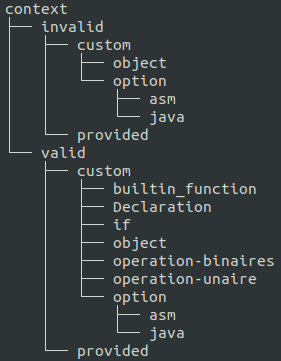
\includegraphics[scale=0.7]{treecontext.png}
    \end{center}


    \subsection{Tests de génération de code avec l'option -java}
    Enfin, concernant les tests de génération de code, nous avons décidé d'utiliser des tests de type "boîte noire".
    Pour chaque fichier de test nous créons un fichier .res avec la sortie attendue. Ainsi, pour chaque test, le script vérifie
    que le résultat obtenu en exécutant le fichier .class avec notre compilateur correspond bien au résultat attendu.
    \begin{flushleft}
        Ces tests se trouvent dans le répertoire \textit{gl28/src/test/deca/codegen}, puis on distingue les tests valides et invalides.
    \end{flushleft}
    \subsubsection{Lancer les tests de génération de code}
    Le script qui permet de lancer l'exécution de tous les tests est \textbf{basic-gencode-java.sh}, il se trouve dans le répertoire \textit{gl28/src/test/script}.
    \begin{flushleft}Les tests sont donc lancés en utilisant l'option -java, ce qui permet de générer des fichiers .class
    exécutables par la JVM. La comparaison entre le résultat obtenu et le résultat attendu nous permet de nous assurer du bon
    fonctionnement de notre extension BYTE. Si le résultat n'est pas le bon, alors un message l'indique.
    \end{flushleft}

    \subsubsection{Arborescence des tests de génération de code}
    Le répertoire \textit{codegen} se trouve dans le dossier \textit{gl28/src/test/deca}. Le rôle de chacun de ces répertoires est expliqué dans la documentation de validation.
    \begin{center}
        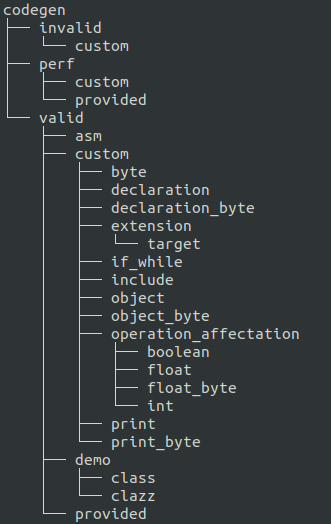
\includegraphics[scale=0.6]{treecodegen.png}
    \end{center}

    \subsubsection{Répertoire \textit{option/java}}
    En particulier, le répertoire \textit{extension} vérifie le bon fonctionnement de l'insertion de code java dans deca. Par exemple, il est possible d'importer une librairie java et de l'utiliser pour retourner un résultat.

    \section{Limitations}
    \subsection{Compilation Deca pour la JVM}
    Il n'y a pas de limitation autre que celle déjà présente pour la compilation IMA.

    \subsection{Insertion de code Java dans Deca}
    L'insertion de code Java en Deca est relativement peu limitée, en effet toute portion de code
    Java-correct pouvant être utilisée dans une méthode sera acceptée et fonctionnelle. Cela comprend donc des
    déclarations de classes, utilisation de packages disponibles etc. Néanmoins, il y a tout de même quelques limitations lié à la syntaxe Deca.

    En effet, les arguments possibles sont limités au types présents dans Deca. Cela vaut également
    pour le type de retour qui doit en plus se limiter aux types primitifs (int, float, boolean). En effet
    pour avoir un type de retour avec objet il faut que ce type existe dans la programme Deca sinon
    la vérification contextuelle bloque avant la génération de code. Puis il faut que la classe soit accessible
    depuis \textbf{$<$nom du ficher deca$>$MethodJavaBodies}. Or la classe existant de manière statique, ce type n'est pas
    associé au "vrai objet" mais à la classe stockant les corps de méthode Java.

    Une autre limitation est qu'il n'est pas possible d'appeler une méthode deca depuis un corps Java. En effet, cela
    pose un problème de nom si deux méthodes ont le même nom dans Deca et dans Java. De plus les corps de méthode Java
    étant séparés des classes principales, le code n'est pas accessible directement. Par contre il est possible d'appeler une
    méthode Java depuis un corps de méthode Java.

    \textbf{\textit{Exemple incorrect}}
    \begin{minted}{java}
        class A {
            void printOk() {
                println("Ok");
            }

            void print java ("
                printOk(); // Incorrect
            ");

        }
    \end{minted}

    \textbf{\textit{Exemple correcte}}
    \begin{minted}{java}
    class A {

        float cos(float x) java ("
            return (float) java.lang.Math.cos(x);
        ");

        float cos2(float x) java ("
            return (float) java.lang.Math.pow(cos(x), 2);
        ");
    }

    {
        A a = new A();
        println(a.cos2(2));
    }
    \end{minted}

    Il est également nécessaire de n'utiliser ces fonctions qu'au sein du même répertoire au risque d'avoir des problèmes d'importation.

    \subsection{Utilisation de programme Deca en Java}
    La compilation pour la JVM mettant actuellement les champs publics, l'encapsulation peut ne pas être conservée lors de l'appelle de programme deca en Java.

    \newpage
    \printbibliography

\end{document}
